\chapter{2024}
\section*{一、程序阅读题}

1. 有一个整数 n, 其中 n 为 2 的幂。程序通过如下代码计算 count 的值, 并返回。请分析并给出该代码的时间复杂度。

\begin{lstlisting}[language=C, basicstyle=\ttfamily]
int main() {
    int count = 0;
    int x = 2;
    while (x < n/2) {
        x = x * 2;
        count++;
    }
    return count;
}
\end{lstlisting}

2. 下面给出一段关于链表操作的代码片段, 请将这些代码片段按正确的顺序排列, 使其实现将结点 \(\mathrm{s}\) 插入到结点 \(\mathrm{p}\) 之前的功能(假设 \(\mathrm{p}\) 既不是头结点也不是尾结点),并分析时间复杂度。代码片段如下:

① prev->next != p \&\& prev->next != NULL

② prev->next = s

③ head == NULL || p == NULL || s == NULL

④ prev->next == p
\begin{lstlisting}[language=C, basicstyle=\ttfamily]
void insertBefore(Node* head, Node* p, Node* s){
    if (______) return;
    Node* prev = head;
    while (______) {
        prev = prev->next;
    }
    if (______) {
        s->next = p;
        ______
    }
}
\end{lstlisting}

\newpage

3. 合并两个非递减的链表为一个非递增链表,以下是部分代码, 请补全代码使其正确实现功能,假设链表的长度分别为 \(\mathrm{n}\) 和 \(\mathrm{m}\) ,分析这段代码的时间复杂度。

\begin{center}
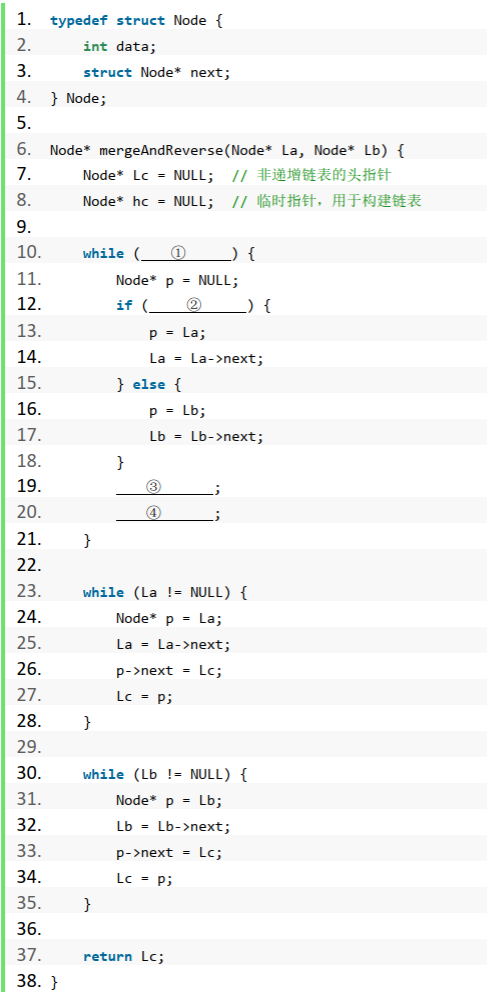
\includegraphics[width=0.6\textwidth]{images/2024/3.png}
\end{center}

4. 请补全下面拓扑排序算法中的代码,假设顶点数为 \(\left| V\right|\) ,边数为 \(\left| E\right|\) ,分析这段代码的时间复杂度。

\begin{lstlisting}[language=C, basicstyle=\ttfamily]
bool Topologicalsort(Graph G) {
    InitStack(S);
    for (int i = 0; i < G.vexnum; i++) {
        if (indegree[i] == 0) {
            ______①______;
        }
    }
    int count = 0;
    while (______②______) {
        ______③______;
        print[count++] = i;
        for (p = G.vertices[i].firstarc; ______④______; p = p->nextarc) {
            v = p->adjvex;
            if (!(--indegree[v])) {
                Push(S, v);
            }
        }
    }
    if (count < G.vexnum) {
        return false;
    } else {
        return true;
    }
}
\end{lstlisting}

\newpage

5. 描述以下递归代码的功能。

\begin{lstlisting}[language=C, basicstyle=\ttfamily]
int func(TreeNode* root) {
    if (root == NULL) {
        return 0;
    }
    if (root->left == NULL && root->right == NULL) {
        return 1;
    }
    return func(root->left) + func(root->right);
}
\end{lstlisting}

\section*{二、填空题}

1. 设循环队列的表长为 \(\mathrm{n},\mathrm{f}\) 指向元素的前一个位置, \(\mathrm{r}\) 指向最后一个元素的位置。该循环队列的长度为\_\_\_\_\_。

2. 将中缀表达式 a+b-a*((c+d)/e-f)+g 转换为后缀表达式\_\_\_\_\_。

3. 给定字符串 abcaabbabcab, 求其对应的 next 数组。

\begin{center}
\begin{tabular}{|c|c|c|c|c|c|c|c|c|c|c|c|c|}
\hline
\phantom{X} & \(\mathbf{a}\) & b & c & a & a & b & b & a & b & c & a & b \\
\cline{1-13}
下标 i & 1 & 2 & 3 & 4 & 5 & 6 & 7 & 8 & 9 & 10 & 11 & 12 \\
\cline{1-13}
next[i] & \phantom{X} & \phantom{X} & \phantom{X} & \phantom{X} & \phantom{X} & \phantom{X} & \phantom{X} & \phantom{X} & \phantom{X} & \phantom{X} & \phantom{X} & \phantom{X} \\
\cline{1-13}
\hline
\end{tabular}
\end{center}

4. 在哈夫曼树中,已知有 1247 个结点,叶子结点的个数为\_\_\_\_\_。

5. 对序列 \(\{ 1,2,3,4,5,6,7\}\) 进行顺序插入构建平衡二叉树,平衡因子为 0 的结点个数为\_\_\_\_\_。

6. 给定一个二维数组 \(\mathrm{A}\left\lbrack  {10}\right\rbrack  \left\lbrack  {15}\right\rbrack  ,\mathrm{A}\left\lbrack  0\right\rbrack  \left\lbrack  0\right\rbrack\) 的地址为 644,行优先存储,每个元素占用一个地址空间, A[4][5]的地址为\_\_\_\_\_。

7. 已知一棵树有 2011 个结点, 其中 116 个是叶结点, 其对应二叉树中右子树为空的结点数量为\_\_\_\_\_。

8. 设森林 F 中有三棵树,第一,第二,第三棵树的结点个数分别为 M1、M2 和 M3。 与森林 F 对应的二叉树根结点的左子树上的结点个数是\_\_\_\_\_。

9. 已知一棵完全二叉树的第六层有 8 个叶结点, 树根位于第一层, 树的最多结点数为\_\_\_\_\_。

\section*{三、综合应用题}

1. 设数组 \(\mathrm{S}\left\lbrack  \right\rbrack   = \{ {93},{946},{372},9,{146},{151},{301},{485},{236},{372},{43},{892}\}\) , (1)采用最低位优先(LSD)基数排序将 S 排列成升序序列。写出每一趟排序的结果。

(2)增量等于 5 时进行希尔排序,写出第一趟排序结果。

(3)以第一个元素为轴进行快速排序,写出第一趟排序结果。

(4)构造小根堆,写出调整后的小根堆。

2. 设散列函数 \(\mathrm{H}\left( \mathrm{{key}}\right)  = \mathrm{{key}}\;\mathrm{MOD}\;{11}\) ,用线性探测再散列法解决冲突。对关键字序列 (13,28,72,5,16,18,7,11,24) 在地址空间为 0-10 的散列区中建散列表, 画出此表, 并求等概率情况下查找成功和查找失败时的平均查找长度。

\begin{center}
\begin{tabular}{|c|c|c|c|c|c|c|c|c|c|c|c|}
\hline
下标 & 0 & 1 & 2 & 3 & 4 & 5 & 6 & 7 & 8 & 9 & 10 \\
\cline{1-12}
关键字 & \phantom{X} & \phantom{X} & \phantom{X} & \phantom{X} & \phantom{X} & \phantom{X} & \phantom{X} & \phantom{X} & \phantom{X} & \phantom{X} & \phantom{X} \\
\cline{1-12}
\hline
\end{tabular}
\end{center}

\newpage
3. 一棵二叉树的先序、中序和后序序列如下, 其中有部分未标出:

先序序列:\_\_\_\_\_ \(\mathrm{{CDE}}\_ \mathrm{{GHI}}\_ \mathrm{K}\)

中序序列:CB \_ FA \_ J K I G

后序序列: \_ \(\mathrm{{EFDB}}\) \_ \(\mathrm{{JIH}}\_ \mathrm{A}\)

(1)根据所给序列补全先序、中序、后序序列。

(2)构造二叉树。

(3)画出二叉树的中序线索链表。

4. 使用弗洛伊德算法,计算下面图的最短路径,给出每一步的最短路径矩阵 \({\mathrm{D}}^{\left( \mathrm{i}\right) }\) 以及保存中转点的矩阵 path \({}^{\left( \mathrm{i}\right) }\) 。

\begin{center}
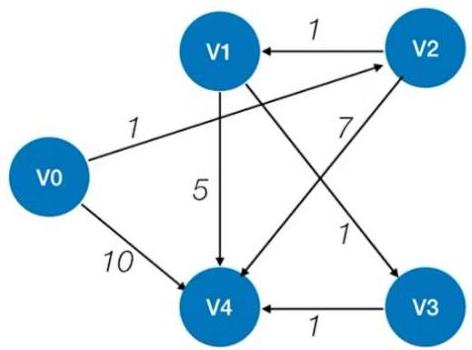
\includegraphics[width=0.6\textwidth]{images/2024/bo_d35pqfjef24c73b45bp0_4_251_309_472_350_0.jpg}
\end{center}

\begin{center}
\begin{tabular}{|c|c|c|c|c|}
\hline
\phantom{X} & \phantom{X} & \phantom{X} & \phantom{X} & \phantom{X} \\
\cline{1-5}
\phantom{X} & \phantom{X} & \phantom{X} & \phantom{X} & \phantom{X} \\
\cline{1-5}
\phantom{X} & \phantom{X} & \phantom{X} & \phantom{X} & \phantom{X} \\
\cline{1-5}
\phantom{X} & \phantom{X} & \phantom{X} & \phantom{X} & \phantom{X} \\
\cline{1-5}
\hline
\end{tabular}
\end{center}

\newpage
5. 设某通信信息由若干字母组成,字母以及其出现的次数如下表所示。 采用赫夫曼(Huffman)编码算法对上述序列编码, 给出相应的 Huffman 树, 以及每个字符的 Huffman 码。

\begin{center}
\begin{tabular}{|c|c|c|c|c|c|c|c|}
\hline
字符 & a & b & c & d & e & f & g \\
\cline{1-8}
出现频率 & 2 & 5 & 6 & 8 & 13 & 19 & 36 \\
\cline{1-8}
\hline
\end{tabular}
\end{center}

6. 对 ["Jan", "Feb", "Mar", "Apr", "May", "Jun", "Jul", "Aug", "Sep", "Oct", "Nov", "Dec"]的月份集合, 执行以下操作:

(1)构造二叉排序树,并计算查找成功的平均查找长度。

(2)对月份简写进行排序后,利用折半查找,计算查找成功的平均查找长度。

(3)构造二叉平衡树,并计算成功的平均查找长度。

\newpage

注: 所有答案必须写在答题纸上, 试卷上作答无效! 第 5 页/共 6 页

重庆邮电大学 2024 年攻读硕士学位研究生入学考试试题(回忆修订版)

\section*{四、算法设计与分析题}

1. 编写代码及思想, 判断一棵树是否为二叉排序树, 结构体已给出。

\begin{lstlisting}[language=C, basicstyle=\ttfamily]
typedef struct BiTNode {
    int data;
    struct BiTNode* lchild;
    struct BiTNode* rchild;
} BiTNode, *BiTree;
\end{lstlisting}

\newpage

2. 编写代码及思想,判断在无向图中是否存在从顶点 \(\mathrm{i}\) 到顶点 \(\mathrm{j}\) 的长度为 \(\mathrm{k}\) 的路径 (使用邻接表表示图)。

\newpage

3. 编写代码及思想, 计算二叉树的繁荣度 (即每一层的结点数乘以该层的层数)。
